\chapter{MỞ ĐẦU}

Trong chương này, chúng tôi trình bày động lực nghiên cứu về quy hoạch tuyến tính và các ứng dụng của nó trong nghiên cứu lý thuyết cũng như thực tiễn. Bên cạnh đó, chúng tôi cũng trình bày tổng quan về lịch sử hình thành và phát triển của lĩnh vực nghiên cứu Toán học này.

\section{Tổng quan về đề tài}

\subsection{Động lực nghiên cứu}

Trong cuộc sống con người, có nhiều bài toán như lập lịch công việc hay canh tác cây trồng nông nghiệp có thể hình thức hóa thành bài toán tối ưu. Bài toán này cực đại hoặc cực tiểu một hàm dưới (các) ràng buộc bất đẳng thức/ đẳng thức, và thường có dạng như sau:

\begin{equation}
    \begin{aligned}
    \min / \max f(x) \\ 
    \text{s.t. } g(x) & \\
    \end{aligned}
\end{equation}
Trong đó: $f(x)$ là hàm mục tiêu, $g(x)$ là ràng buộc (bất đẳng thức/ đẳng thức)

Và trong trường hợp đơn giản nhất, hàm mục tiêu là hàm tuyến tính và các ràng buộc là ràng buộc tuyến tính. Đây là bài toán quy hoạch tuyến tính hay tối ưu tuyến tính.

\subsection{Ý nghĩa khoa học - thực tiễn ứng dụng}

Quy hoạch tuyến tính được sử dụng nhiều trong lĩnh vực tối ưu hóa. Nhiều vấn đề trong nghiên cứu vận trù học cũng được khai triển về dạng bài toán quy hoạch tuyến tính để tăng tốc thời gian giải và giảm độ phức tạp bài toán. Hơn nữa, trong các lĩnh vực nghiên cứu khác như lý thuyết đồ thị cũng tận dụng kỹ thuật này để giải quyết một số bài toán như luồng trong mạng.

Trong ứng dụng thực tiễn, quy hoạch tuyến tính được sử dụng để giải quyết nhiều bài toán quản lý cho doanh nghiệp như lập lịch, hay vận chuyển nguyên liệu. Cụ thể, Google sử dụng kỹ thuật này để ổn định đề xuất cho các videos Youtube.

\subsection{Những đóng góp của tiểu luận}

\subsection{Cấu trúc của tiểu luận}

Nội dung nghiên cứu của tiểu luận được trình bày trong bảy chương:
\begin{itemize}
    \item Chương 1 - Mở đầu
    \item Chương 2 - Mô hình bài toán
    \item Chương 3 - Phương pháp hình học cho bài toán quy hoạch tuyến tính hai biến
    \item Chương 4 - Phương pháp đơn hình
    \item Chương 5 - Phương pháp lập trình cho quy hoạch tuyến tính
    \item Chương 6 - Một số ứng dụng của quy hoạch tuyến tính
    \item Chương 7 - Kết luận và hướng nghiên cứu tương lai
\end{itemize}

\section{Lịch sự hình thành và phát triển}

\epigraph{"A certain wide class of practical problems appears to be just beyond the range of modern computing machinery. These problems occur in everyday life; they run the gamut from some very simple situations that confront an individual to those connected with the national economy as a whole. Typically, these problems involve a complex of different activities in which one wishes to know which activities to emphasize in order to carry out desired objectives under known limitations."
\\ \underline{Tạm dịch}: Một lớp các bài toán thực tế cụ thể nhất định nằm ngoài khả năng tính toán của máy tính hiện đại. Những bài toán này xuất hiện mọi lúc trong đời sống hằng ngày; chúng có thể nằm trong một số tình huống hết sức đơn giản hoặc thậm chí là liên quan đến toàn bộ nền kinh tế quốc gia. Thông thường, những bài toán này phát sinh một chuỗi phức tạp các mục tiêu khác nhau mà trong đó người ta mong muốn biết cần tối đại mục tiêu nào trong những giới hạn cho trước.
}{George B. Dantzig, 1948}

\subsection{Trước những năm 1930}

Vào những năm 1827, Jean-Baptiste Joseph Fourier đã công bố phương pháp giải hệ bất đẳng thức tuyến tính - một trong những vấn đề toán học đã có từ rất lâu về trước. Sau này,  Theodore Motzkin đã khám phá lại phương pháp và phát triển thuật toán mà ngay nay ta biết đến với tên gọi phép khử Fourier–Motzkin.

Trong những năm 1930, nhà toán học Liên Xô Leonid Kantorovich và nhà kinh tế học người Mỹ Tjalling Charles Koopmans đã độc lập nghiên cứu các ứng dụng của quy hoạch tuyến tính. Họ đã cùng nhau đưa LP lên một tầm cao mới bằng cách chứng minh những ứng dụng rộng rãi của nó trong các vấn đề phân phối tài nguyên, và lập lịch sản xuất. Sau này, họ cùng nhau nhận giải Nobel Kinh tế vào năm 1975.

Năm 1941, Frank Lauren Hitchcock cũng đã thành công trong việc xây dựng các bài toán vận tải như quy hoạch tuyến tính và đưa ra phương án giải quyết tương tự như phương pháp đơn hình sau này. Tuy nhiên, ông đã qua đời và giải Nobel không thể trao cho ông.

\subsection{Thời kỳ sơ khai (1947 - 1990)}

Trong những năm 1946 - 1947, nhà toán học người Mỹ George Bernard Dantzig\footnotemark{} đã làm việc độc lập để xây dựng phương pháp quy hoạch tuyến tính tổng quát trong bài toán lập lịch bay cho không quân Hoa Kỳ. Vào năm 1947, ông đã đề xuất phương pháp đơn hình - phương pháp có thể giải quyết hầu hết các bài toán mà hình thức hóa thành dạng bài toán quy hoạch tuyến tính. Điều này về cơ bản đã cách mạng hóa việc sử dụng quy hoạch tuyến tính trong thực tế.

\footnotetext{Dantzig được biết đến với việc giải quyết hai vấn đề mở chưa có lời giải trong lĩnh vực thống kê, nhầm chúng với bài tập về nhà sau khi đến giảng muộn tại trường Đại học Berkeley.}

Sau đó, vào mùa thu năm 1947, Jack Laderman thuộc Dự án Mathematical Tables Project of the National Bureau of Standards đã sử dụng phương pháp đơn hình trong việc giải bài toán ăn kiêng\footnotemark{} và kiểm chứng mô hình của George Stigler. Đây là dự án tính toán quy mô lớn đầu tiên của lĩnh vực tối ưu hóa, bài toán quy hoạch tuyến tính gồm 9 phương trình với 77 biến ẩn. Trong quá trình thực hiện, dự án cần chín nhân viên sử dụng máy tính để bàn vận hành bằng tay và mất 120 ngày công để tìm ra giải pháp tối ưu là 39,69 USD. Dự đoán của Stigler chỉ sai lệch 0,24 USD mỗi năm!

\footnotetext{Bài toán ăn kiêng là một trong những bài toán tối ưu hóa đầu tiên được nghiên cứu vào những năm 1930 và 1940. Vấn đề được thúc đẩy bởi mong muốn của Quân đội nhằm giảm thiểu chi phí cho lính GI ăn tại thực địa trong khi vẫn cung cấp chế độ ăn uống lành mạnh. Một trong những nhà nghiên cứu đầu tiên nghiên cứu vấn đề này là George Stigler, người đã đưa ra phỏng đoán có căn cứ về giải pháp tối ưu bằng phương pháp heuristic. Dự đoán của ông về chi phí cho một chế độ ăn tối ưu là 39,93 USD mỗi năm (giá năm 1939).}

Vào năm 1951, mã nguồn máy tính cho quy hoạch tuyến tính lần đầu tiên được công bố bởi National Bureau of Standards (bây giờ được gọi là NIST) được chạy trên máy tính SEAC. Với một bài toán LP 48 phương trình và 71 biến ẩn, máy tính cần 18 giờ và 73 lần lặp đơn hình để có thể đưa ra lời giải tối ưu. Đến năm 1954, Card Programmable Calculator được tạo ra. Thời gian để giải một bài toán LP với 26 phương trình và 71 biến ẩn giảm xuống còn 8 tiếng.

Một cách tóm tắt sự phát triển trong những năm 1955 - 1973:
\begin{itemize}
    \item 1954-55: IBM 701, 100-200 rows
    \item 1956: IBM 704, 4 K "core", RSLP1, 255 rows
    \item 1962-66: 7090/94, LP/90/94, 1024 rows
    \item 1966-70: IBM 360, MPS/360 \& MPSX/370 giải hệ LP thực đầu tiên.
    \item 1971-73: MPS III/Whizard, 32000 rows
\end{itemize}

Trong thập kỷ 70, sự quan tâm dành cho nghiên cứu và ứng dụng của tối ưu hóa trở nên lớn. Điều này được thể hiện ở việc nhiều các ứng dụng lập lịch ở quy mô lớn được phát triển và tài nguyên đầu tư nghiên cứu trở nên nhiều hơn. Tuy nhiên, nhiều khó khăn và thách thức đã xuất hiện:
\begin{itemize}
    \item Chi phí xây dựng hệ thống ứng dụng rất tốn kém và đầy rủi ro.
    \item Chu kỳ phát triển dự án rất dài, từ 3-4 chu kỳ.
    \item Các nhà lập trình và chủ sở hữu đối mặt với nhiều vấn đề chuyên môn như: máy tính, dữ liệu, thuật toán và kỹ thuật mô hình hóa.
    \item Công nghệ tính toán chưa sẵn sàng.
\end{itemize}
Thế nên, sự phát triển của LP (MIP cũng gặp tình trạng tương tự) gặp trở ngại, kéo theo đó là sự vỡ mộng và phần lớn sự vỡ mộng đó vẫn còn tồn tại cho đến ngày nay.

Đến giữa thập kỷ 80, người ta cho rằng LP đã phát triển đến hết mức có thể, đỉnh cao nhất thời điểm hiện tại có lẽ là MPSX/370 và MPSIII. Nhưng LP chắc chắn không phải là một vấn đề được giải quyết… ví dụ: Mô hình LP của hãng hàng không “Không thể giải quyết được” với 4420 ràng buộc, 6711 biến. Tuy vậy, trong thời gian này cũng có nhiều sự phát triển đáng chú ý:
\begin{itemize}
    \item Máy tính IBM được giới thiệu vào năm 1981.
    \item Cơ sở dữ liệu quan hệ được phát triển.
    \item Chứng minh được LP có thể giải được trong thời gian đa thức.
    \begin{itemize}
        \item Năm 1979, Khachiyan chỉ ra rằng LP có thể giải được trong thời gian đa thức bằng "phương pháp ellipsoid". Đây là một bước đột phá về mặt lý thuyết hơn là một bước đột phá thực tế, vì trong thực tế, thuật toán khá chậm.
        \item Năm 1984, Karmarkar đã phát triển "phương pháp điểm trong", một thuật toán thời gian đa thức khác cho LP, cũng hiệu quả trong thực tế. Cùng với phương pháp đơn hình, đây là phương pháp được lựa chọn ngày nay để giải LP.
    \end{itemize}
\end{itemize}

Trong thời gian này, lý thuyết vận trù học có nhiều bước phát triển, đặc biệt là lý thuyết matroid. Từ những năm 1983, ngay sau khi công bố giới thiệu máy tính, IBM bắt đầu phát triển mã nguồn LP. Vào năm 1985 - 1987, Tom Baker đã giới thiệu mã nguồn LP cho sản phẩm Chesapeake Decision Sciences MIMI. Và mãi đến 1988, IBM CPLEX được thành lập. 

Cho đến cuối thập kỷ 80 này, LP vẫn chưa thoát khỏi bế tắc. Một số bài toán quy hoạch tuyến tính trở nên rất khó giải, ngay cả đối với các bộ giải LP thương mại được đánh giá cao như MPSX của IBM. Các bài toán LP có ~1500 phương trình và ~2500 biến và mất gần 3 giờ để giải nếu chúng giải được. Và kèm theo đó là sự thoái hóa, hội tụ chậm và tính không linh hoạt của hệ thống vẫn là những trở ngại lớn trong các bộ giải tối ưu thương mại.

\begin{figure}[h!]
    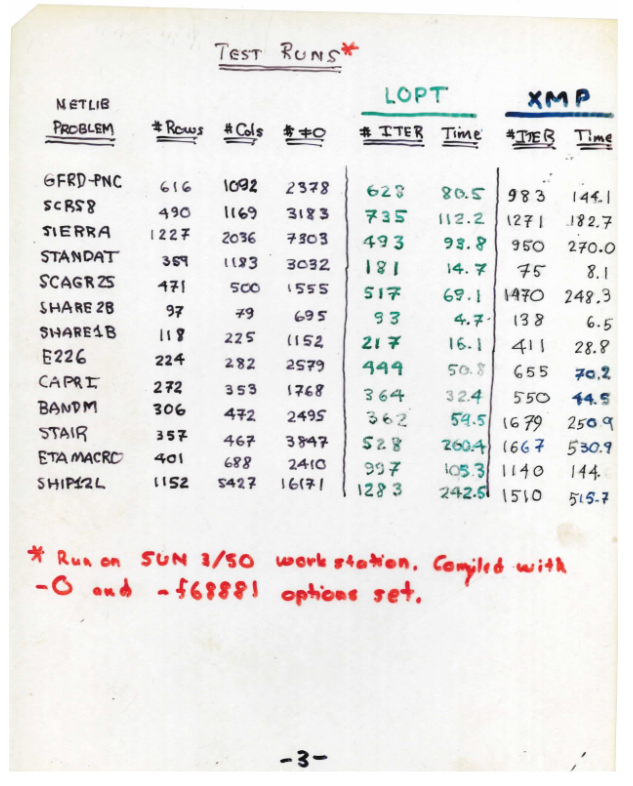
\includegraphics[width=0.85\linewidth]{figures/cplex_1986.png}
    \caption{Kết quả bộ giải CPLEX vào năm 1986.}
    \label{fig:cplex_1986}
\end{figure}

Đến những năm của thập kỷ 90, nhiều bước tiến mới đã giúp LP cải thiện đáng kể về mặt hiệu năng và mở rộng thêm nhiều hướng ứng dụng mới. Các phương pháp primal-dual log-barrier đã nâng cao tốc độ giải LP. Bên cạnh đó dữ liệu cũng trở nên đa dạng và dễ dàng truy cập được. Thế nên có nhiều ứng dụng mới từ các bài toán thực tế bắt đầu cho thấy tính khả thi của việc ứng dụng quy hoạch tuyến tính và quy hoạch nguyên như hàng không, hay chuỗi cung ứng.

\subsection{Những bước phát triển mới}

\subsubsection{AA Challenge,}

\subsubsection{AA \& US Air Merger,}

\subsubsection{LAU2} Là một bài toán phân công đội tàu

\subsection{Quy hoạch tuyến tính ngày nay}

\subsubsection{Mô hình lập lịch thương mại}

Bài toán lập lịch là bài toán quan trọng và được quan tâm bởi doanh nghiệp. Trong thương mại, các bộ giải LP đối mặt với bài toán với 401640 ràng buộc, 1584000 biến. Dưới đây là đánh giá với bộ giải CPLEX qua các năm.

\begin{table}[h!]
    \caption{Test.}
    \centering
    \begin{tabular}{llcc}
        \hline
        Năm &  Bộ giải &  Thời gian & Tốc độ cải thiện  \\
        \hline
        1988 & CPLEX 1.0 & 29.8 ngày & 1x \\
        1997 & CPLEX 5.0 & 1.5 giờ & 480x \\ 
        2003 & CPLEX 9.0 & 59.1 giây & 43500x \\ 
        \hline
    \end{tabular}
\end{table}

\subsubsection{Tiến triển trong LP giai đoạn 2004 - 2015}